\documentclass{article}
\usepackage[utf8]{inputenc}
\usepackage{amsmath}
\usepackage{listings}
\usepackage[norsk]{babel}
\usepackage{graphicx}
\usepackage{float}

\title{Oblig 1b: Analyse av Terningdropp}
\author{Gormery Kombo}
\date{\today}

\begin{document}

\maketitle

\section{Introduksjon}
I denne rapporten analyserer jeg data samlet fra et eksperiment hvor en terning ble droppet fra ulike høyder. jeg undersøker sammenhengen mellom høyden terningen ble sluppet fra (Dropp) og lengden den rullet (Lengde) etter å ha truffet bakken. Analysen inkluderer regresjonsanalyse og residualanalyse for å forstå forholdet mellom disse variablene.

\section{Oppgave 2}
\subsection{2a: Datainnsamling og Analyse}
Dataene som ble samlet inn er tilgjengelige i filen \texttt{terningDropp.csv}. Dataene ble analysert ved hjelp av R for å utføre statistiske beregninger og visuelle representasjoner.

\subsection{2b: Regresjonsanalyse for de Første 5 Målingene}
Først ble det utført en regresjonsanalyse på de første fem målingene for å estimere sammenhengen mellom 'Dropp' og 'Lengde'. Resultatene gir oss en innsikt i hvordan lengden varierer med høyden i de første forsøkene.

\begin{lstlisting}[language=R]
lm_first5 <- lm(Lengde ~ Dropp, data=df[1:5, ])
summary(lm_first5)
\end{lstlisting}
\textbf{Regresjonslinje (2b):} Resultatene fra R er sammenlignet med manuell beregning for å sikre nøyaktighet.

\subsection{2c: Regresjonsanalyse for Hele Datasettet}
Deretter ble en lignende regresjonsanalyse utført på hele datasettet for å se om det samme mønsteret holder for en større mengde data.

\begin{lstlisting}[language=R]
lm_full <- lm(Lengde ~ Dropp, data=df)
\end{lstlisting}

\subsection{2d: Spreddiagram av Data}
Følgende spreiddiagram viser alle datapunktene (Dropp mot Lengde) fra eksperimentet. Dette gir oss en visuell representasjon av datadistribusjonen.

\begin{figure}[H]
    \centering
    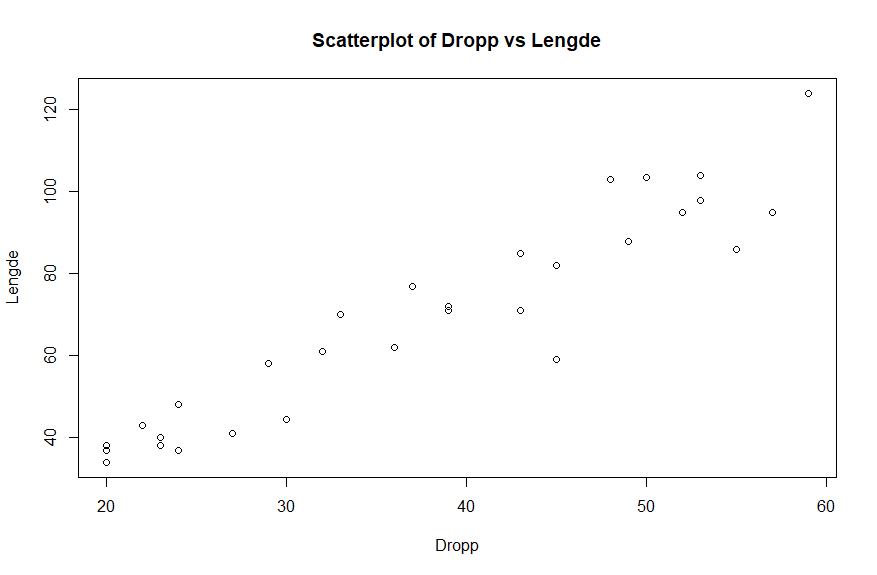
\includegraphics[width=0.8\textwidth]{Rplot03.png}
    \caption{Spreddiagram av Dropp mot Lengde (2d)}
\end{figure}

\subsection{2e: Spreddiagram med Regresjonslinje}
Dette spreiddiagrammet inkluderer regresjonslinjen som viser den estimerte lineære sammenhengen mellom 'Dropp' og 'Lengde' for hele datasettet.

\begin{figure}[H]
    \centering
    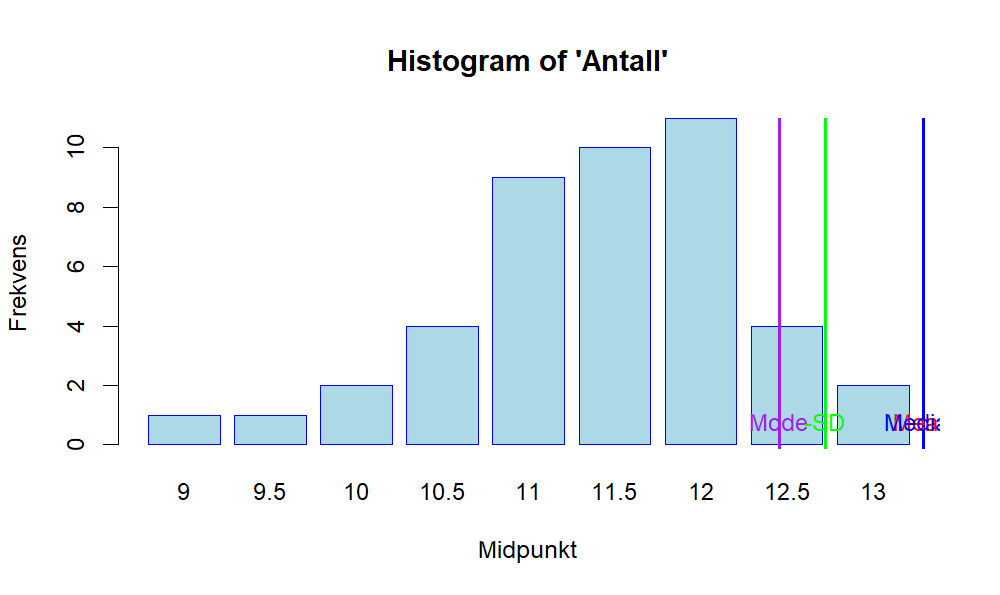
\includegraphics[width=0.8\textwidth]{Rplot02.png}
    \caption{Spreddiagram med regresjonslinje (2e)}
\end{figure}

\subsection{2g: Sum av Kvadrerte Residualer (SSe)}
Summen av de kvadrerte residualene (SSe) gir oss en kvantitativ måling av hvor godt regresjonsmodellen passer dataene. Lavere verdier indikerer en bedre passform.

\begin{lstlisting}[language=R]
ssr_first5 <- sum(residuals(lm_first5)^2)
ssr_full <- sum(residuals(lm_full)^2)
\end{lstlisting}
\textbf{SSR (2g):} SSR for de første 5 målingene: \[ 748.808  \]
SSR for hele datasettet: \[ 2114.794 \]

\subsection{2h: Standardfeil (se)}
Standardfeilen (SE) gir oss en idé om usikkerheten i estimatet av regresjonskoeffisientene. Den hjelper oss å forstå hvor nøyaktig vår lineære modell estimerer den avhengige variabelen.

\begin{lstlisting}[language=R]
se_first5 <- sqrt(ssr_first5 / lm_first5$df.residual)
se_full <- sqrt(ssr_full / lm_full$df.residual)
\end{lstlisting}
\textbf{Standardfeil (2h):} SE for de første 5 målingene: \[ 15.79882 \]
SE for hele datasettet: \[ 8.690704 \]

\subsection{2i: Lagring av Arbeid (for meg selv)}
Jeg Lagret det utførte arbeidet som en r prosject på github: \\ 
\texttt{https://github.com/valiantlynx/statistics-course/tree/main/statistikk-oblig-1b}

\end{document}
